\section{Interaktion der Komponenten}
Auf Basis der Analyse Use Cases wird in diesem Kapitel die Interaktion der einzelnen Komponenten aus Kapitel 1 betrachtet. 
Dabei liegt der Fokus vor allem der Interaktion zwischen der RobotUnit und dem Server, wie dessen Austausch mit dem Hospital und der Taxiapp. 
Die Abläufe innerhalb der Komponenten werden dann in Kapitel 8 näher spezifiziert. \\


\subsection*{Interaktion bei Ausführung von \emph{Receive Order \& Cancel Order}}

Elementar ist in diesem Fall der UseCase ReceiveOrder(Use Case 1.1), der es Usern ermöglicht Anfragen oder Notrufe aufzusetzen, um ein Taxi oder einen Krankentransporter anzufordern. 
Das System arbeitet mit einer Warteliste; Krankentransporter werden in jedem Fall priorisiert und es wird schnellstmöglich die nächste RobotUnit zur Verfügung gestellt. 
Im Falle des ersten Sequenzdiagramm ist dies mit der Verwendung der Taxiapp dargestellt, die wiederum die Zielkoordinate Destination an den Server weitergibt. 
Danach wird vom Server überprüft, ob überhaupt Taxis verfügbar sind, um schließlich ein Warteplatz an die App zurückgegeben, der an den User weitergeleitet wird. 
Mit Cancel Order(Use Case 1.2) können sich User dabei jederzeit aus der Warteliste streichen lassen. 
Im Falle des Krankentransporters existiert diese Warteliste nur in theoretischer Natur. 
Sie wird, wie im zweiten Sequenzdiagramm ersichtlich, nicht über das Hospital an den User zurückgegeben, sondern es wird ein Krankentransporter ein Krankentransporter, sobald ein RobotUnit verfügbar ist. \\

\begin{figure}[H]
	\centering
	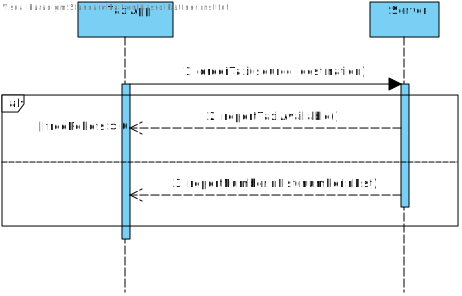
\includegraphics[width=0.9\textwidth]{img/2-Entwurf-RecieveOrder-Taxi}
	\caption{\emph{RecieveOrder-Taxi}-Sequenzdiagramm}
	\label{SequenzDiagrammInteraktion}
\end{figure}

\begin{figure}[H]
	\centering
	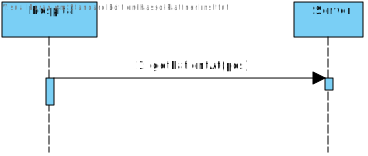
\includegraphics[width=0.9\textwidth]{img/2-Entwurf-RecieveOrder-Hosp}
	\caption{\emph{SEntwurf-RecieveOrder-Hosp}-Sequenzdiagramm}
	\label{SequenzDiagrammInteraktion}
\end{figure}



\subsection*{Interaktion bei Ausführung von \emph{Receive Boarding Confirmation \& Receive Arrival Notification}}

Alle Prozesse laufen wie ersichtlich über den Server, der wiederum die RobotUnit fernsteuert. 
So wird sowohl für Receive Boarding Confirmation( Use Case 1.3) erst vom Hospital oder der TaxiApp an den Server zurückgemeldet, dass sich der Patient oder der Costumer an Bord befindet, bevor die Fahrt aufgenommen werden kann. 
In gleichem Weise wird dem Server mit Receive Arrival Notification(UseCase 1.5) zurückgemeldet,das die RobotUnit wieder für weitere Einsätze verfügbar ist, sobald der Costumer die RobotUnit verlassen hat.  \\

\begin{figure}[H]
	\centering
	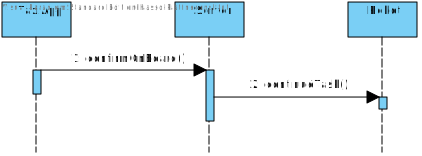
\includegraphics[width=0.9\textwidth]{img/2-Entwurf-ReceiveBoardingConfirmation-taxi}
	\caption{\emph{ReceiveBoardingConfirmation-taxi}-Sequenzdiagramm}
	\label{SequenzDiagrammInteraktion}
\end{figure}

\begin{figure}[H]
	\centering
	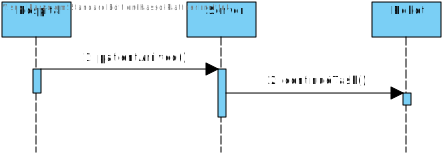
\includegraphics[width=0.9\textwidth]{img/2-Entwurf-ReceiveUnloadConfirmation-hospital}
	\caption{\emph{ReceiveUnloadConfirmation-hospital}-Sequenzdiagramm}
	\label{SequenzDiagrammInteraktion}
\end{figure}


\subsection*{Interaktion bei Ausführung von \emph{Use Cases Perfom Task \& Continue Task}}
Konkret wird die RobotUnit dabei über die UseCases Perfom Task(Use Case 2.2) und Continue Task( Use Case 2.3) eine Task(Parameter) zugewiesen, die solange ausgeführt, bis der der RobotUnit eine Abbruch Task zugewiesen wird oder das Ziel wiederum erfolgreich erreicht wurde und dies an den Server zurückgemeldet werden kann. \\

\begin{figure}[H]
	\centering
	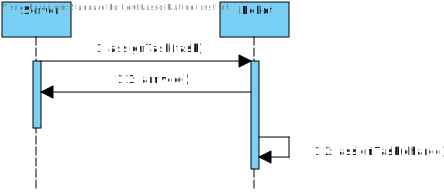
\includegraphics[width=0.9\textwidth]{img/2-Entwurf-Perform Task}
	\caption{\emph{Perform Task}-Sequenzdiagramm}
	\label{SequenzDiagrammInteraktion}
\end{figure}

\subsection* Die weiteren UseCases sind diesen untergeordnet; enthalten entweder nur einseitige Server/RobutUnit Kommunikation, wie zum Beispiel bei Request Repair( Use Case 1.6) oder haben ihren Fokus vor allem auf den Wechselwirkungen innerhalb der Robot Unit( Siehe dazu Kapitel 8). \\

